\section{Support Vector Machine (SVM)}

\subsection{1. Review of SVM Strategies}
\textbf{Task:} Summarize OvR vs OvO and choose suitable strategy.

\paragraph{Answer.}
Support Vector Machines are fundamentally binary classifiers, but multi-class classification can be handled through decomposition strategies:
\begin{itemize}
  \item \textbf{One-vs-Rest (OvR):} train \(K\) classifiers for \(K\) classes; each classifier separates one class from all remaining classes.
  \item \textbf{One-vs-One (OvO):} train \(\frac{K(K-1)}{2}\) pairwise classifiers and aggregate predictions by voting.
\end{itemize}

In scikit-learn, \texttt{LinearSVC} typically uses OvR, while \texttt{SVC} uses OvO internally. For the digits dataset, both are valid: OvR is computationally efficient, while OvO with kernels can better model nonlinear boundaries.

\subsection{2. Regularization Parameter}
\textbf{Task:} Explain role of C and other tunable parameters.

\paragraph{Answer.}
The soft-margin parameter \(C\) controls the bias-variance trade-off:
\begin{itemize}
  \item \textbf{Small \(C\):} stronger regularization, wider margin, more tolerated training errors, risk of underfitting.
  \item \textbf{Large \(C\):} weaker regularization, fewer tolerated errors, narrower margin, risk of overfitting.
\end{itemize}

For RBF SVM, \(\gamma\) is also critical:
\begin{itemize}
  \item \textbf{High \(\gamma\):} highly flexible and localized decision boundary.
  \item \textbf{Low \(\gamma\):} smoother and more global boundary.
\end{itemize}
Good performance requires tuning both \(C\) and (for kernels) \(\gamma\).

\subsection{3. Linear SVM Experiment}
\textbf{Task:} Train/validate over logarithmic C grid and discuss validation accuracy.

\paragraph{Answer.}
With an 80\%/20\% train-validation split on the digits dataset and \(C\) values swept logarithmically from \(10^{-4}\) to \(10^{4}\), the best reported linear-SVM validation accuracy is:
\[
0.9694 \quad (96.94\%) \text{ at } C=0.1.
\]

For very small \(C\), regularization is too strong and the model underfits. As \(C\) increases, accuracy improves and reaches a maximum near \(C=0.1\). Beyond that point, performance slightly decreases and stabilizes around \(0.947\), consistent with mild overfitting for overly large \(C\).

\subsection{4. Kernel SVM Experiment}
\textbf{Task:} Repeat with RBF kernel and compare to linear SVM.

\paragraph{Answer.}
Repeating the same \(C\) sweep with an RBF kernel yields low accuracy for very small \(C\) (around 20\%), then strong improvements as \(C\) increases. The best reported result is:
\[
0.9806 \quad (98.06\%) \text{ at } C=10.
\]

Comparison with linear SVM:
\begin{itemize}
  \item Linear best: \(0.9694\)
  \item RBF best: \(0.9806\)
\end{itemize}

The RBF model performs better, indicating that the digits data is not perfectly linearly separable. This improvement is explained by the kernel trick, which implicitly maps samples to a higher-dimensional feature space where more complex class boundaries can be represented.

\begin{figure}[h]
  \centering
  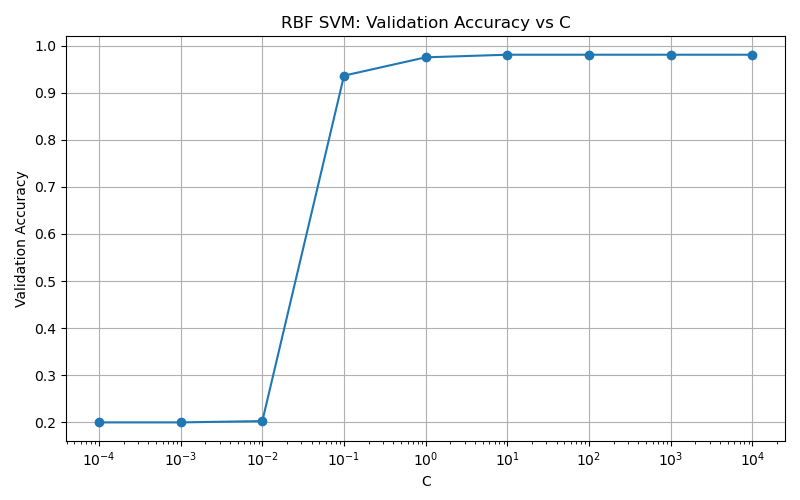
\includegraphics[width=0.78\textwidth]{figures/svm_graph.png}
  \caption{SVM validation performance across regularization settings.}
  \label{fig:svm_graph}
\end{figure}
